\textbf{ID:} UC04 (Create Event)
\textbf{Scope}: CS Automated Information Timeline\\
\textbf{Level}: User Goal\\
\textbf{Stakeholders and Interests}:
\begin{itemize}
        \item Faculty: A person that works for the university and is interested in gaining visibility of their post and/or event.
        \item Admin/Reviewer: A person that works for the university and approves and/or removes posts and/or events from the system.
\end{itemize}
\textbf{Preconditions}:
\begin{itemize}
    \item Faculty has been identified and authenticated.
\end{itemize}
\textbf{Postconditions}:
    \begin{itemize}
    \item Event has been persisted.
    \item Event has been placed in the proposed state.
    \item An event notification has been persisted.
\end{itemize}
\textbf{Main Success Scenario}:
\begin{enumerate}
    \item Faculty writes the event using the event creation tool.
    \begin{enumerate}
        \item The event title is written by the faculty user.
        \item The event body is written by the faculty user.
    \end{enumerate}
    \item Faculty reviews the event draft.
    \item Faculty submits the event to the system.
    \begin{enumerate}
        \item An event id is generated by the system.
        \item A timestamp is generated by the system.
        \item The user id of the faculty user is attached to the event object.
        \item The system assigns the status of the event to the proposed state.
    \end{enumerate}
    \item The system generates a notification object.
    \begin{enumerate}
        \item The event object is attached to the notification object.
    \end{enumerate}
    \item The notification object is persisted.
    \item The event object is persisted.
    \item The system returns the persisted event object to the faculty user.
\end{enumerate}
\textbf{Extensions:}
\begin{enumerate}
    \item[*.a.] Anytime the system does not respond,
    \begin{enumerate}
        \item[1.] Faculty will notify the Admin/Reviewer.
        \item[2.] Admin/Reviewer will restart the system.
    \end{enumerate}
    \item [5.a.] If the notification is not persisted,
    \begin{enumerate}
        \item [1.] The system returns an error message to the faculty user.
        \item[2.] The faculty user resubmits the event.
    \end{enumerate}
    \item [6.a.] If the event is not persisted,
    \begin{enumerate}
        \item [1.] The system returns an error message to the faculty user.
        \item [2.] Faculty reattempts the submission of the event.
    \end{enumerate}
\end{enumerate}

\begin{figure}[H]
    \centering
    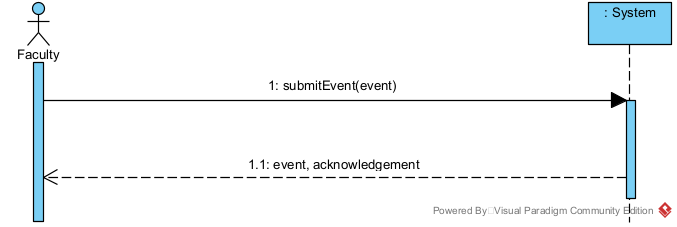
\includegraphics[width=0.8\textwidth]{images/SSD-UC04-CreateEvent.png}
    \centering
    \caption{System Sequence Diagram: Create Event}
\end{figure}

\textbf{Operation:} submitEvent(event: Event) \\
\textbf{Cross References:} UC04 (Create Post) \\
\textbf{Preconditions:}
\begin{itemize}
    \item Faculty, f, has been identified and authenticated.
\end{itemize}
\textbf{Postconditions:}
\begin{itemize}
    \item Event, e, was created.
    \item Event e.status was set to “proposed”.
    \item Event, e, was persisted.
\end{itemize}